\begin{frame}
  \frametitle{Expected activation levels}
  %% \framesubtitle{}

  \begin{itemize}
  \item Since we are interested in the general behaviour of a stochastic NDL, it makes sense to average over many individual learners to obtain \primary{expected associations} $\bigExp{V_j\psupt}$
  \end{itemize}

  \[
  \bigExp{V_{j+1}\psupt} = \bigExp{V_j\psupt} + \bigExp{\Delta V_j\psupt}
  \]

  \ungap[.5]
  \begin{align*}
    \bigExp{\Delta V_j\psupt} 
    &= \Expscale{ 
      c_i \beta \bigl( o - \textstyle\sum_{j=1}^n c_j V_j\psupt \bigr)
      } \qquad\qquad\qquad\qquad \\
    & \only<beamer:2| handout:0>{
      = \beta\cdot \bigExp{c_i o} - \beta\cdot \Expscale{c_i \textstyle\sum_{j=1}^n c_j V_j\psupt}
      }%
      \only<beamer:3| handout:0>{
      = \beta\cdot \bigExp{c_i o} - \beta\cdot \textstyle\sum_{j=1}^n \secondary{\bigExp{c_i c_j V_j\psupt}}
      }%
      \only<beamer:4| handout:0>{
      = \beta\cdot \secondary{\bigExp{c_i o}} - \beta\cdot \textstyle\sum_{j=1}^n \secondary{\bigExp{c_i c_j}} \bigExp{V_j\psupt}
      }% 
      \only<beamer:5| handout:1>{
      = \beta\cdot\left( \p{C_i, O} - \textstyle\sum_{j=1}^n \p{C_i, C_j} \bigExp{V_j\psupt} \right)
      }% 
  \end{align*}

  \begin{itemize}
  \item<3-> $c_i$ and $c_j$ are independent from $V_j$
  \item<4-> indicator variables: $\Exp{c_i o} = \p{C_i, O}$; $\Exp{c_i c_j} = \p{C_i, C_j}$
  \end{itemize}
\end{frame}

\begin{frame}
  \frametitle{Expected activation levels}
  %% \framesubtitle{}
  
  \ungap[1.5]
  \[
  \only<beamer:1-5| handout:0>{\Delta V_j\psupt = c_i\psupt \beta \bigl( o\psupt - \textstyle\sum_{j=1}^n c_j\psupt V_j\psupt \bigr)}%
  \only<beamer:6-| handout:1>{\bigExp{\Delta V_j\psupt} = \beta\cdot\bigl( \p{C_i, O} - \textstyle\sum_{j=1}^n \p{C_i, C_j} \bigExp{V_j\psupt} \bigr)}%
  \]
  
  \centering
  \only<beamer:1| handout:0>{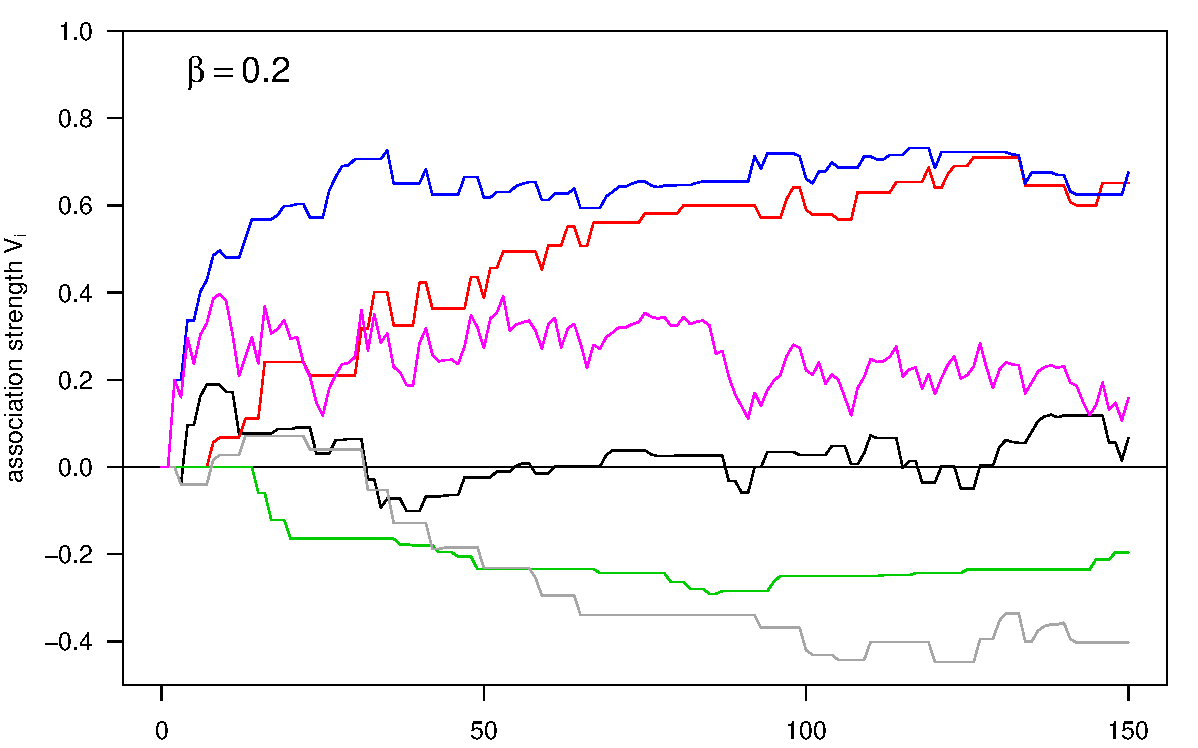
\includegraphics[width=10cm]{img/german_plural_exp_rw_step_1}}%
  \only<beamer:2| handout:0>{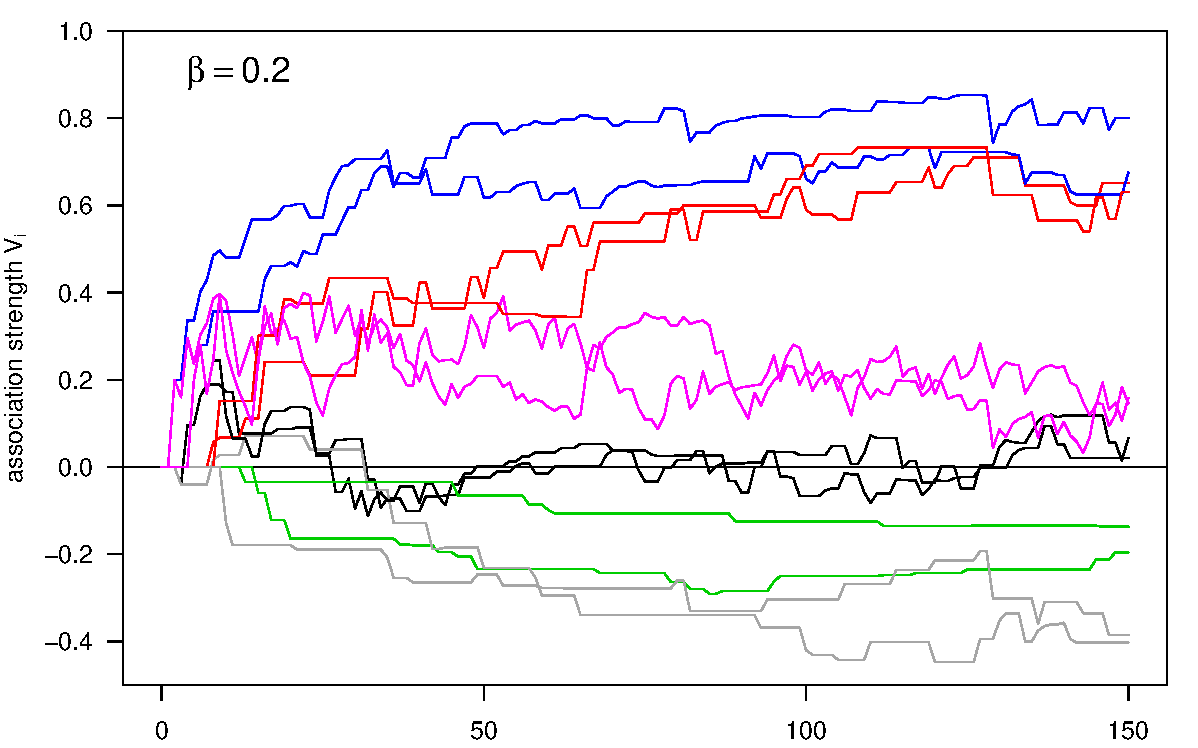
\includegraphics[width=10cm]{img/german_plural_exp_rw_step_2}}%
  \only<beamer:3| handout:0>{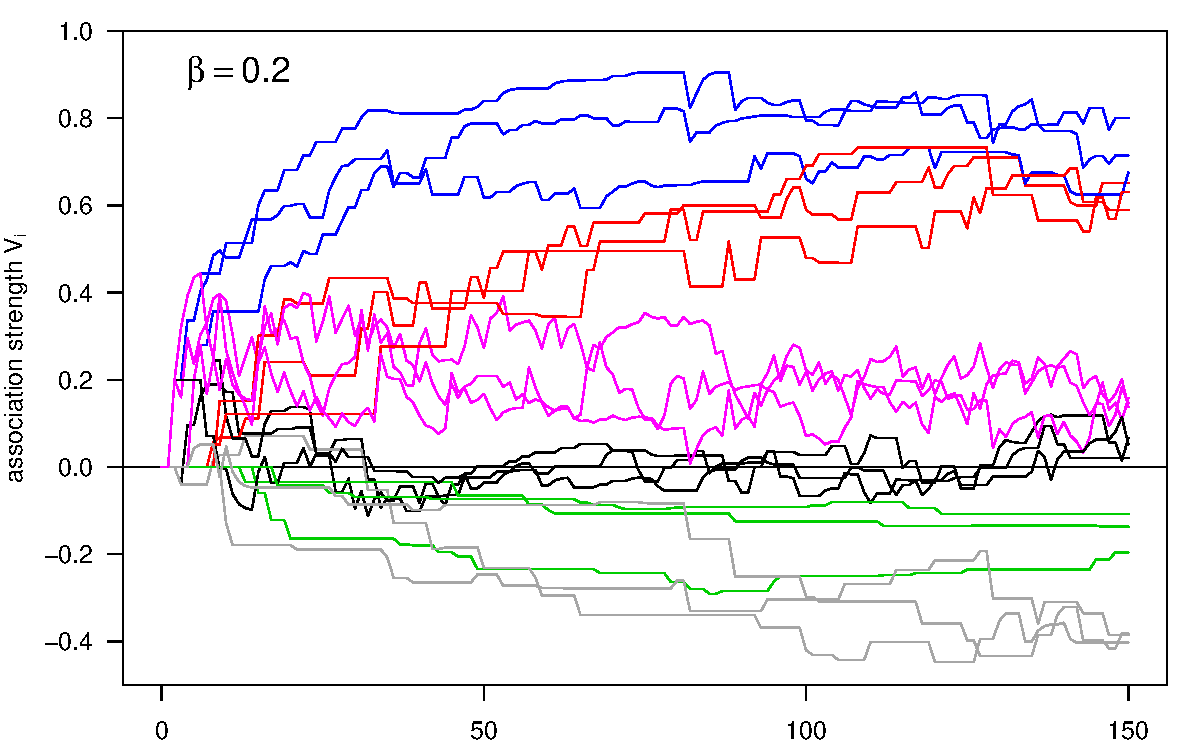
\includegraphics[width=10cm]{img/german_plural_exp_rw_step_3}}%
  \only<beamer:4| handout:0>{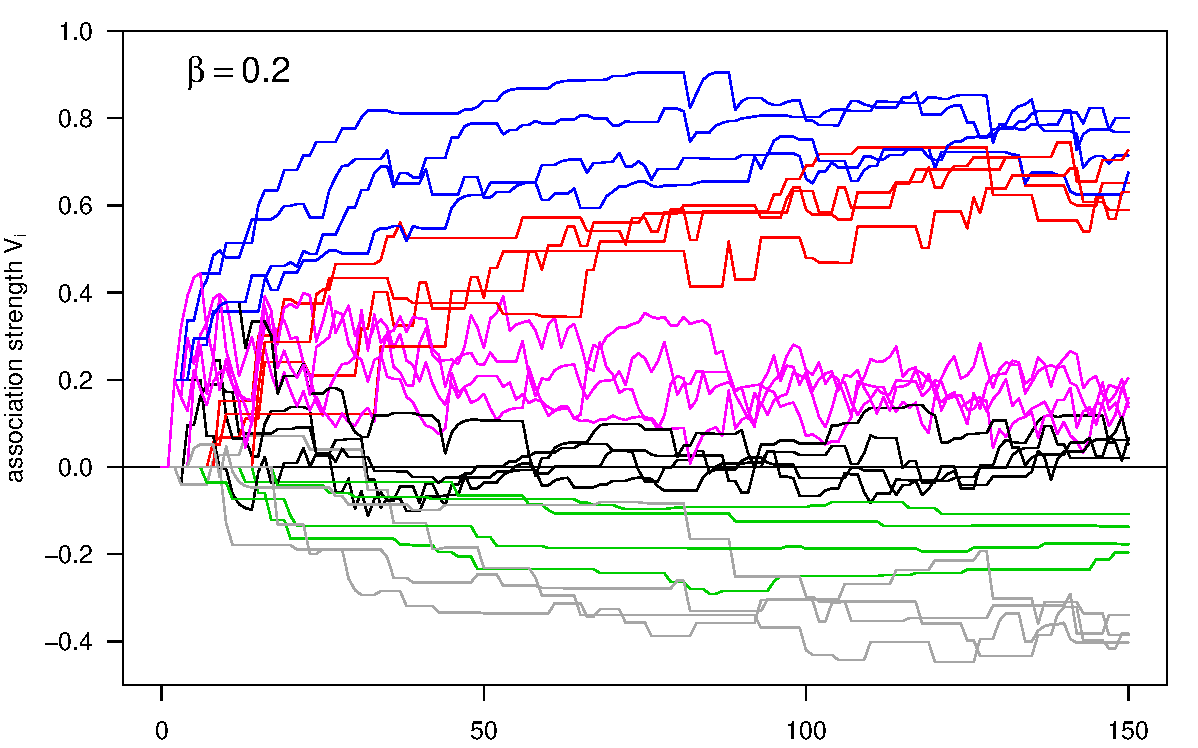
\includegraphics[width=10cm]{img/german_plural_exp_rw_step_4}}%
  \only<beamer:5| handout:0>{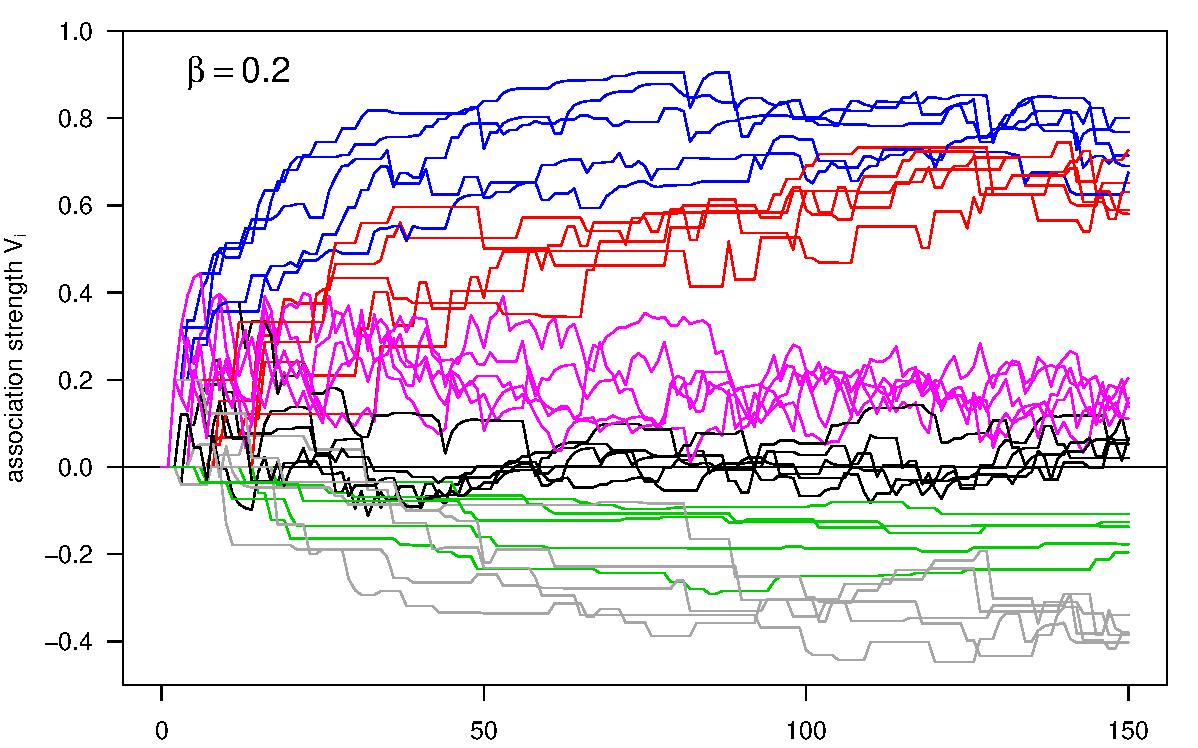
\includegraphics[width=10cm]{img/german_plural_exp_rw_step_5}}%
  \only<beamer:6| handout:1>{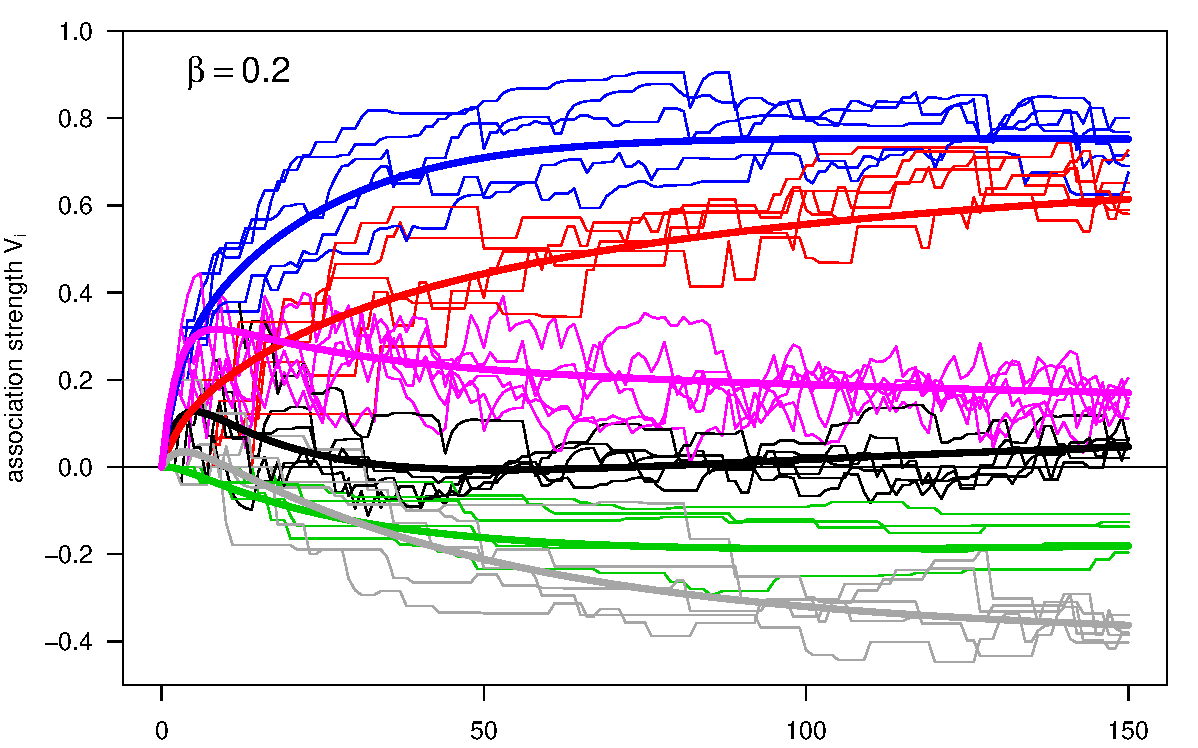
\includegraphics[width=10cm]{img/german_plural_exp_rw_final}}%
\end{frame}

\begin{frame}
  \frametitle{The Danks equilibrium}
  %% \framesubtitle{}

  \begin{itemize}
  \item If $\bigExp{V_i\psupt}$ converges, the asymptote $V_i^* = \lim_{t\to \infty} \bigExp{V_i\psupt}$ must satisfy the \primary{Danks equilibrium} conditions $\bigExp{\Delta V_i^*} = 0$:
    \[
    \p{C_i, O} - \textstyle\sum_{j=1}^n \p{C_i, C_j} V_j^* = 0
    \]
    \citep[p.~113]{Danks:03}
  \item This equation allows us to compute the stable ``adult'' state of the learner without carrying out a simulation of the learning process (either stochastic NDL or expected values)
  \end{itemize}
\end{frame}

\begin{frame}[c]
  \frametitle{The Danks equilibrium}
  %% \framesubtitle{}

  \centering
  \only<beamer:1| handout:1>{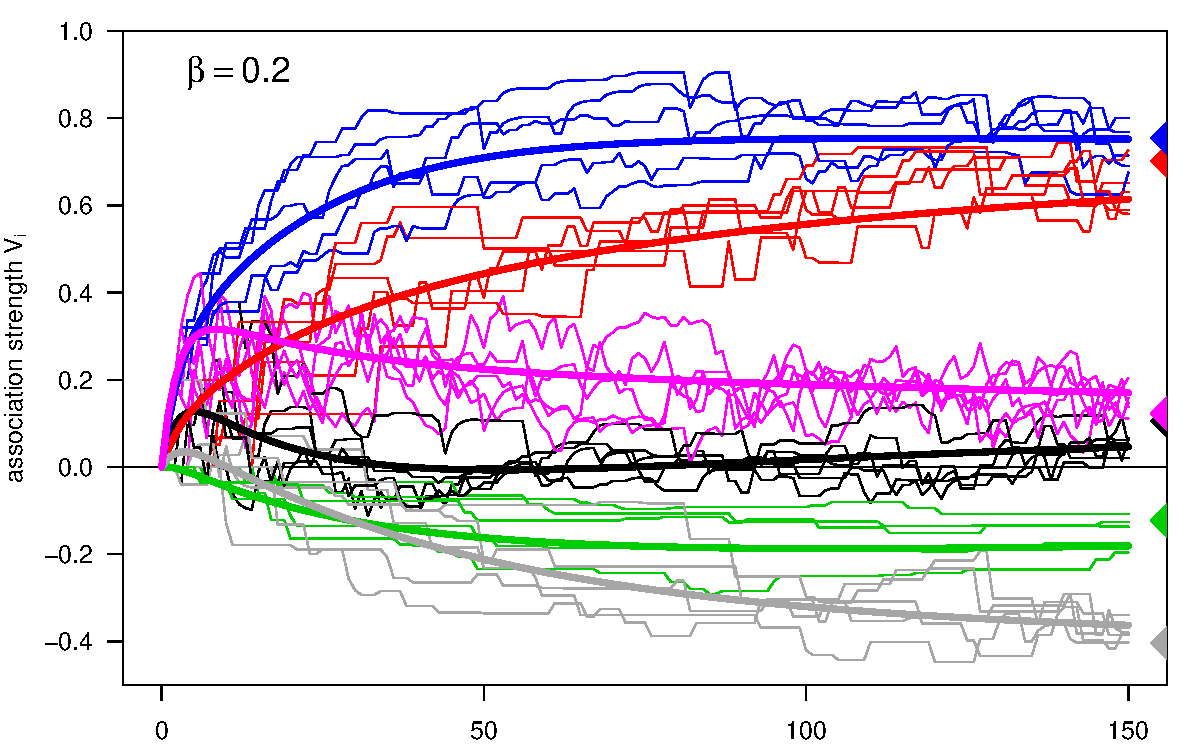
\includegraphics[width=11cm]{img/german_plural_exp_rw_danks}}%
  \only<beamer:2| handout:0>{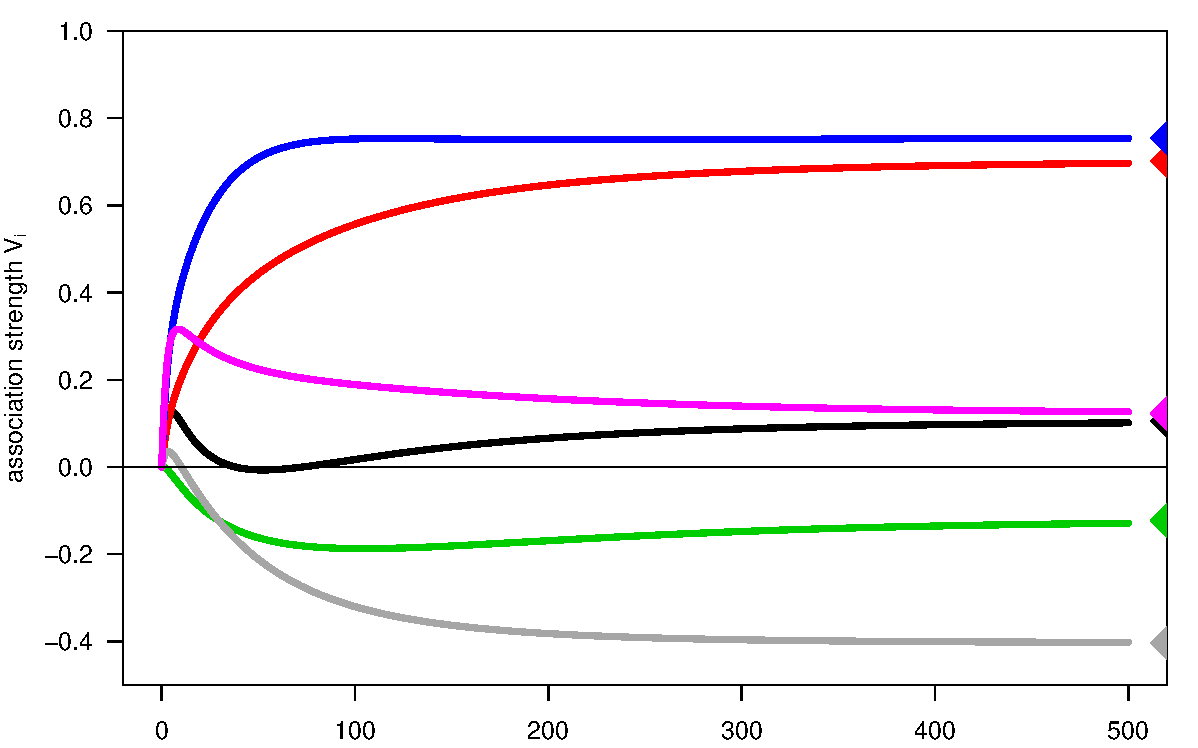
\includegraphics[width=11cm]{img/german_plural_exp_rw_danks_500}}%
\end{frame}

\begin{frame}
  \frametitle{Matrix notation}
  %% \framesubtitle{}
  
  \ungap[2]
  \begin{align*}
    \vX &=
    \begin{bmatrix}
      c_1\psup{1} & \cdots & c_n\psup{1} \\
      c_1\psup{2} & \cdots & c_n\psup{2} \\
      \vdots      &        & \vdots      \\
      c_1\psup{m} & \cdots & c_n\psup{m} 
    \end{bmatrix}
    &
    \vz &=
    \begin{bmatrix}
      o\psup{1} \\
      o\psup{2} \\
      \vdots \\
      o\psup{m}
    \end{bmatrix}
    &
    \vw &=
    \begin{bmatrix}
      V\psup{1} \\
      \vdots \\
      V\psup{n}
    \end{bmatrix}
  \end{align*}
  
  \begin{align*}
    \only<beamer:2-3| handout:0>{
    \small\begin{bmatrix} 
      f(C_1, O) \\ 
      \vdots \\
      f(C_n, O) 
    \end{bmatrix}
    &= \vX^T \vz
    &
    \visible<3->{
    \small\begin{bmatrix} 
      f(C_1, C_1) & \cdots & f(C_1, C_n) \\ 
      \vdots      &       & \vdots \\
      f(C_n, C_1) & \cdots & f(C_n, C_n)
    \end{bmatrix}
    &= \vX^T \vX
    }}%
    \only<beamer:4-| handout:1>{
    \small\begin{bmatrix} 
      \p{C_1, O} \\ 
      \vdots \\
      \p{C_n, O}
    \end{bmatrix}
    &= \tfrac{1}{m} \vX^T \vz
    &
    \small\begin{bmatrix} 
      \p{C_1, C_1} & \cdots & \p{C_1, C_n} \\ 
      \vdots      &       & \vdots \\
      \p{C_n, C_1} & \cdots & \p{C_n, C_n}
    \end{bmatrix}
    &= \tfrac{1}{m} \vX^T \vX
    }
  \end{align*}
  
  \gap[1]
  \[
  \visible<5->{\text{\primary{Danks equilibrium:}}} \quad
  \only<beamer:5| handout:0>{\tfrac{1}{m} \vX^T \vz - \tfrac{1}{m} \vX^T \vX \vw^* = \vnull}%
  \only<beamer:6-| handout:1>{\vX^T \vz = \vX^T \vX \vw^*}%
  \]
\end{frame}

\begin{frame}
  \frametitle{Matrix notation: German noun plurals}
  %% \framesubtitle{}
  
  \ungap[2]
  \begin{align*}
    \vX &=
    \footnotesize\begin{bmatrix}
      1 & 0 & 0 & 1 & 0 & 1 \\ 
      1 & 0 & 0 & 0 & 0 & 1 \\ 
      0 & 0 & 0 & 0 & 0 & 1 \\ 
      0 & 0 & 0 & 1 & 0 & 1 \\ 
      0 & 1 & 0 & 0 & 0 & 1 \\ 
      1 & 0 & 0 & 0 & 1 & 1 \\ 
      0 & 1 & 0 & 1 & 1 & 1 \\ 
      0 & 0 & 1 & 0 & 0 & 1 \\      
      1 & 0 & 0 & 1 & 0 & 1 \\ 
      1 & 0 & 0 & 1 & 0 & 1
    \end{bmatrix}
    &
    \vz &=
    \footnotesize\begin{bmatrix}
      1  \\
      0  \\
      0  \\
      1  \\
      1  \\
      0  \\
      1  \\
      0  \\
      1  \\
      1 
    \end{bmatrix}
    &
    \vw &=
    \begin{bmatrix}
      V\psup{1} \\
      \vdots \\
      V\psup{n}
    \end{bmatrix}
  \end{align*}
  
  \begin{align*}
    \only<beamer:1-3| handout:0>{
    \visible<2->{
    \small\begin{bmatrix} 
      3 \\ 
      2 \\
      0 \\
      5 \\
      1 \\
      6
    \end{bmatrix}
    &= \vX^T \vz}
    &
    \visible<3->{
    \small\begin{bmatrix} 
      5 & 0 & 0 & 3 & 1 &  5 \\ 
      0 & 2 & 0 & 1 & 1 &  2 \\ 
      0 & 0 & 1 & 0 & 0 &  1 \\ 
      3 & 1 & 0 & 5 & 1 &  5 \\ 
      1 & 1 & 0 & 1 & 2 &  2 \\ 
      5 & 2 & 1 & 5 & 2 & 10 
    \end{bmatrix}
    &= \vX^T \vX}
    }%
    \only<beamer:4-| handout:1>{
    \small\begin{bmatrix} 
      .3 \\ 
      .2 \\
      .0 \\
      .5 \\
      .1 \\
      .6
    \end{bmatrix}
    &= \tfrac{1}{m} \vX^T \vz
    &
    \small\begin{bmatrix} 
      .5 & .0 & .0 & .3 & .1 &  .5 \\ 
      .0 & .2 & .0 & .1 & .1 &  .2 \\ 
      .0 & .0 & .1 & .0 & .0 &  .1 \\ 
      .3 & .1 & .0 & .5 & .1 &  .5 \\ 
      .1 & .1 & .0 & .1 & .2 &  .2 \\ 
      .5 & .2 & .1 & .5 & .2 &  1 
    \end{bmatrix}
    &= \tfrac{1}{m} \vX^T \vX
    }
  \end{align*}
\end{frame}

%%% Local Variables: 
%%% mode: latex
%%% TeX-master: "../qitl6_evert_arppe"
%%% End: 
